\section{Case Study Artifacts}
\label{app:example_artifacts}

To illustrate the stepwise transformations of our generation pipeline, we present the concrete artifacts generated for the Alternating Bit Protocol (ABP) case study. This section follows the chronological execution of the pipeline, demonstrating how unstructured natural language is progressively refined into a rigorous, executable DEVS model. 


% You can refer to \url{https://demo1.devs-demo.workers.dev} for a better structured detailed example for the StrategicAirlift. 

\subsection{Input Specifications}
\label{app:artifacts_input}
The pipeline begins with the user-provided specifications. Listing \ref{lst:behavioral_spec} defines the operational logic and constraints in natural language, while Listing \ref{lst:operational_spec} dictates the simulation's interface, I/O formats, and configuration parameters. Notably, these inputs contain no explicit DEVS architectural blueprints.

\begin{lstlisting}[caption={Behavioral Specification}]
### Scenario: Reliable Data Transfer with Deterministic Noise Interference
1. System Objective: Design a communication system consisting of a Sender, a Receiver, and two uni-directional transmission channels (Subnets). The goal is to transmit a sequence of packets reliably using an Alternating Bit Protocol (ABP) despite deterministic packet loss in the channels.

2. Entity Behaviors:
The Sender:
    - Accepts a single control input at the start of simulation: the total number of packets to send.
    - Before sending each packet, the Sender must undergo a preparation delay (default 10ms, configurable via --sender_delay).
    - The Receiver must maintain a buffer with capacity 1. During the busy period, it must buffer the only received packet, and process the packet immediately after the busy processing delay. When multiple packets arrive, only the first one is stored.
    - Sends packets sequentially through Subnet1. Each packet contains a sequence number (1, 2, ...) and a control bit (alternating between 0 and 1). The first bit is 0.
    - After sending a packet, it starts a timer (default 20ms, configurable via --timeout).
    - Stop-and-Wait Logic: It must not send the next packet until it receives a correct Acknowledgment (ACK) for the current one.
    - Retransmission: If the timer expires before a valid ACK is received, the Sender retransmits the same packet and restarts the timer.
    - Validation: An ACK is valid only if its bit matches the control bit of the current packet.
    - After sending the specified total number of packets, the Sender stops automatically.

The Receiver:
    - Upon receiving a packet, it undergoes a processing delay (default 10ms, configurable via --receiver_delay) before processing.
    - The Receiver must maintain a buffer with capacity 1. During the busy period, it must buffer the only received packet, and process the packet immediately after the busy processing delay. When multiple packets arrive, only the first one is stored.
    - After the processing delay, it extracts the control bit and immediately sends back an ACK packet containing that same bit through Subnet2.

The Subnets (Channels):
    - There are two independent channels: Subnet1 (Sender -> Receiver) and Subnet2 (Receiver -> Sender).
    - Latency: Every packet takes exactly 3ms (configurable via --channel_delay) to traverse.
    - Deterministic Noise & Loss Model: Each subnet independently simulates interference using a deterministic formula.
        - Each Subnet maintains an internal "noise level" value x, initialized to exactly the seed value (provided via --seed).
        - Packet Fate Determination: When a packet arrives at a subnet, calculate a new noise level: x_new = (17 * x_old + 11) mod 100.
        - If x_new < 10, the interference is too high, and the packet is dropped (vanishes). Otherwise, it is transmitted normally after the channel delay.
        - After determination, update the noise level for the next packet: x_old = x_new.
        - Timing: The noise calculation and fate determination happen immediately when the packet arrives at the subnet.

3. Scenario Constraints:
    - Time Unit Mapping: 1.0 simulation time unit = 1 Millisecond (ms).
    - System starts at time 0.0 with all components initialized to idle states.
\end{lstlisting}
\begin{lstlisting}[caption={Operational Specification}]
1. Command Line Arguments:
The script must accept the following named arguments:
* `--total_packets` (int): The total number of packets the Sender intends to send in one session triggered by a START_BATCH command. 
* `--seed` (int): The initialization seed for the noise generator of both sides (the `x` value in the LCG formula). Default: 42.
* `--timeout` (int): Sender's timeout duration in ms. Default: 20.
* `--sender_delay` (int): Sender preparation delay in ms. Default: 10.
* `--receiver_delay` (int): Receiver processing delay in ms. Default: 10.
* `--channel_delay` (int): Subnet transmission delay in ms. Default: 3.
* `--simulate_time` (int): The total simulation time to run in ms. Default: 1000.

2. stdin Format:
* No stdin input is required for this simulation. The system uses command line arguments for configuration.

3. **Standard Output (stdout)**:
* Format: JSONL, one independent JSON object per line
* Each record MUST follow the format: `{"time": <float>, "entity": <str>, "event": <str>, "payload": <dict>}`
* **Event Types and Formats**:
    Sender Events:
    - event: `delay_start` (Sender starts preparation delay)
    - time: Sender's current time
    - entity: `"sender"`
    - payload: `{"type": "preparation", "duration": <float>}`
    - Trigger: When Sender starts preparing a packet
    
    - event:  `packet_sent` (Packet sent)
    - time: Sender's current time
    - entity: `"sender"`
    - payload: `{"seq_num": <int>, "bit": <0|1>, "is_retry": <bool>}`
    - Trigger: When Sender completes preparation delay and hands packet to subnet
    
    - event: `ack_received` (ACK received)
    - time: Sender's current time
    - entity: `"sender"`
    - payload: `{"ack_bit": <0|1>, "is_valid": <bool>}`
    - Trigger: When Sender receives an ACK
    
    Receiver Events:
    - event: `delay_start` (Receiver starts processing delay)
    - time: Receiver's current time
    - entity: `"receiver"`
    - payload: `{"type": "processing", "duration": <float>}`
    - Trigger: When Receiver starts processing a received packet
    
    - event: `packet_received` (Packet successfully received)
    - time: Receiver's current time
    - entity: `"receiver"`
    - payload: `{"seq_num": <int>, "bit": <0|1>}`
    - Trigger: When Receiver completes processing delay and successfully receives packet
    
    Subnet Events:
    - event: `packet_get` (Packet fate determined)
    - time: Subnet's current time
    - entity: `"subnet"`
    - payload: `{"behavior": <"drop"|"pass">, "channel": <"forward"|"backward">, "noise_value": <int>}`
    - Trigger: When packet arrives at subnet, before transmission delay starts
    - Note: "forward" for Sender->Receiver channel, "backward" for Receiver->Sender channel
\end{lstlisting}

\subsection{Planning Skeleton}\label{app:planning_skeleton_artifact}

The first major transformation extracts a conceptual DEVS hierarchy from the unstructured text. As shown in Listing \ref{lst:spec_skeleton}, the pipeline identifies not only the core physical entities (Sender, Receiver, Subnets) but also intelligently deduces the need for auxiliary utility models, such as \texttt{DelayScheduler} and \texttt{TimeoutTimer}, to handle the temporal constraints specified in the prompt. This step establishes the structural boundaries before detailed logic is generated.

\begin{lstlisting}[language=JSON, caption={The skeleton of the ABP\_Sender}, label={lst:spec_skeleton}]
{
  "modules": [
    {
      "name": "ABP_D1",
      "description": "Top-level DEVS model implementing the Alternating Bit Protocol. Data flow (IC): ABP_Sender sends packets to a forward DeterministicLossSubnet, which passes them to ABP_Receiver; ABP_Receiver sends ACKs to a backward DeterministicLossSubnet, which returns them to ABP_Sender. It also couples shared DelayScheduler and TimeoutTimer components.",
      "children_names": [
        "ABP_Sender",
        "ABP_Receiver",
        "DeterministicLossSubnet",
        "DelayScheduler",
        "TimeoutTimer"
      ]
    },
    {
      "name": "ABP_Sender",
      "description": "Coupled model representing the Sender role. Data flow (IC): ABP_SenderController coordinates internal timing by sending requests to DelayScheduler (for preparation) and TimeoutTimer, routing their timeouts back to the controller. EIC/EOC map external packet/ACK flows.",
      "children_names": [
        "ABP_SenderController",
        "DelayScheduler",
        "TimeoutTimer"
      ]
    },
    {
      "name": "ABP_Receiver",
      "description": "Atomic model handling packet reception. Maintains a capacity-1 buffer, undergoes deterministic processing delay, and generates ACK echoes back to the sender.",
      "children_names": []
    },
    {
      "name": "DeterministicLossSubnet",
      "description": "Atomic model simulating a unidirectional network channel. Receives packets/ACKs, determines deterministic drop fate based on noise seed, and outputs surviving packets after a fixed transmission delay.",
      "children_names": []
    },
    {
      "name": "DelayScheduler",
      "description": "Utility atomic model for scheduling delays. Receives start requests and emits corresponding completion signals after configured sender or receiver delays.",
      "children_names": []
    },
    {
      "name": "TimeoutTimer",
      "description": "Utility atomic model for timeout logic. Receives start/restart requests for outstanding packets and emits a timeout expiration event when the duration elapses.",
      "children_names": []
    },
    {
      "name": "ABP_SenderController",
      "description": "Atomic model executing the core stop-and-wait state machine for the sender. Handles sequence numbers, bit alternation, retransmission logic, and validates ACKs without directly managing the time progression.",
      "children_names": []
    }
  ]
}
\end{lstlisting}

\subsection{Structured PlanTree}
\label{app:artifacts_plan}
Once the skeleton is established, the pipeline performs a top-down refinement to generate the \plantree{}, transforming conceptual modules into strict structural contracts. Figure \ref{fig:plantree_viz} illustrates the resulting hierarchical decomposition.

To demonstrate the rigidity of these contracts, Listing \ref{lst:spec_snippet} provides a condensed view of the \texttt{ABP\_Sender} node. In this phase, ambiguous natural language is translated into explicitly defined I/O ports, data structures, and state initialization parameters. By strictly defining the schemas (e.g., ensuring \texttt{in\_ack} only accepts \texttt{\{'ack\_bit': int\}}), the \plantree{} ensures that downstream code generation for each component can occur in parallel without integration conflicts.

\begin{figure*}[h]
\centering
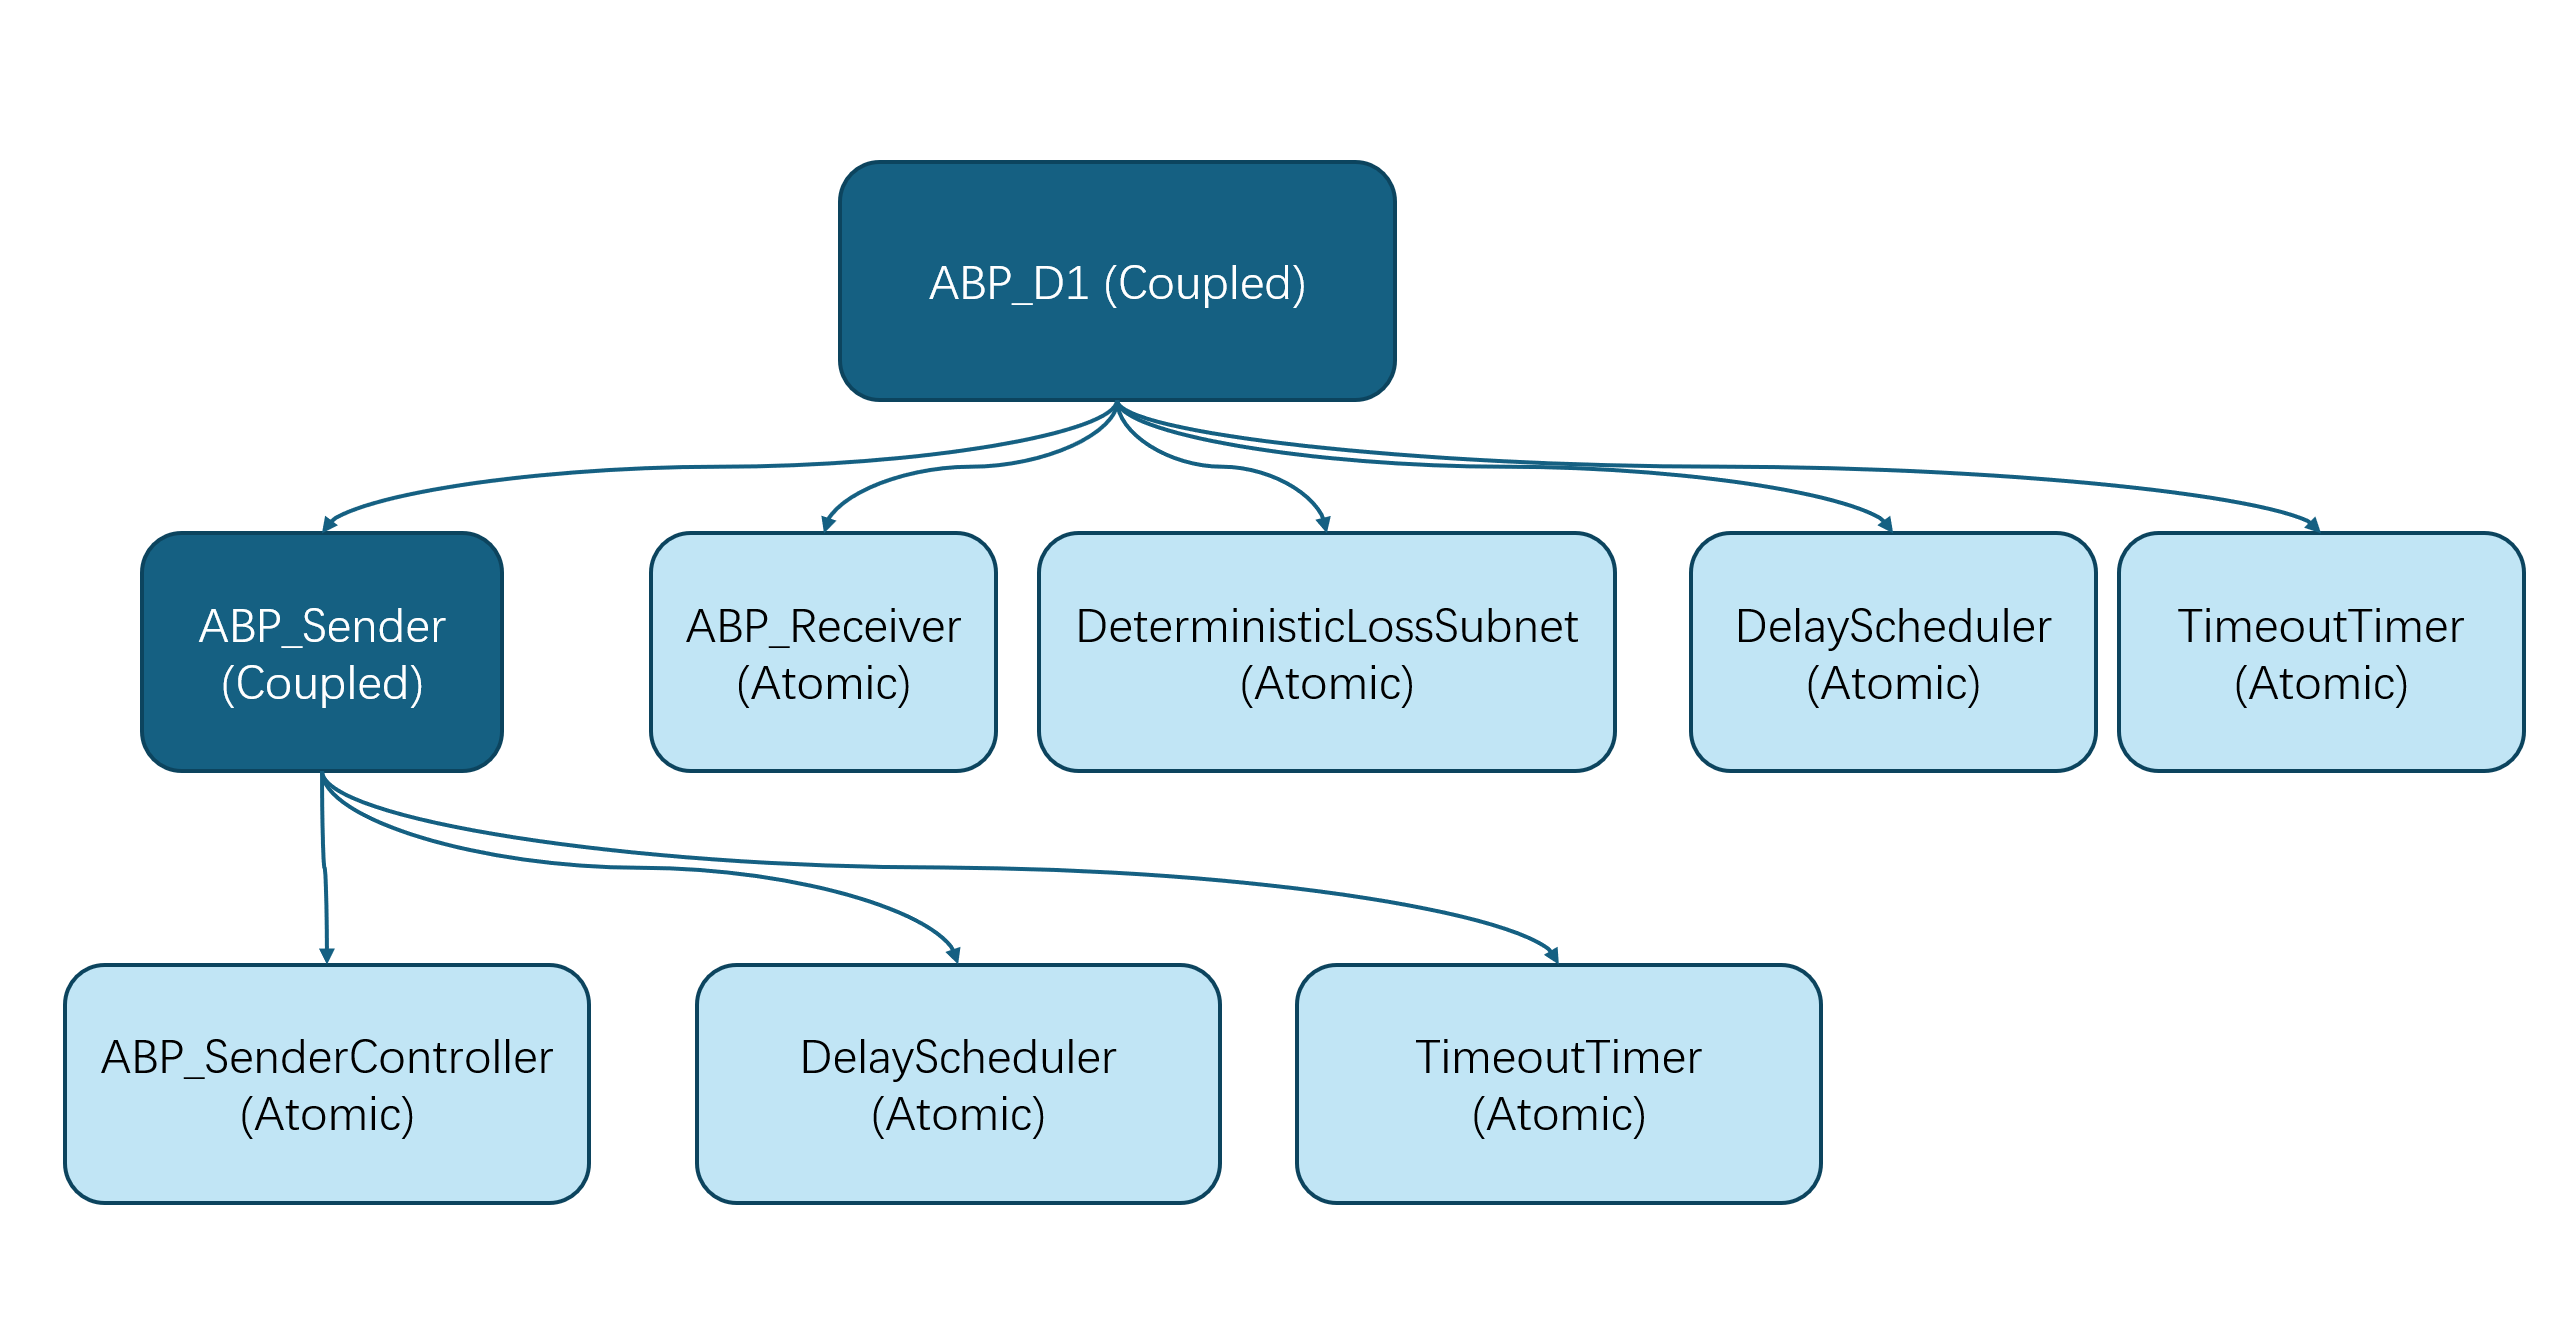
\includegraphics[width=0.85\textwidth]{imgs/abp_plan.png}
\caption{Visualized \plantree{} hierarchy for the ABP Model. The root model recursively decomposes into sub-models until atomic primitives are reached.}
\label{fig:plantree_viz}
\end{figure*}

\begin{lstlisting}[language=JSON, caption={Fragment of the PlanTree focusing on the ABP\_Sender's ModelPlan}, label={lst:spec_snippet}]
{
  "class_name": "ABP_Sender",
  "plan_phase": {
    "type": "coupled",
    "model_info": {
      "specification": {
        // Functional logic extracted from natural language
        "function": "Implements Sender role... [Details Omitted] ...",
        
        // Strict Interface Definitions
        "model_init_args": [
          {"name": "total_packets", "type": "int", "structure": "..."},
          {"name": "timeout", "type": "float", "structure": "..."}
        ],
        
        // Explicit Port Definitions with Protocol
        "input_ports": [
          {
            "name": "in_start",
            "type": "dict",
            "structure": "{'total_packets': int}",
            "protocol": {
              "description": "Optional start command...",
              "initial_signal": "If total_packets>0, auto-start at t=0..."
            }
          },
          {
            "name": "in_ack", 
            "type": "dict", 
            "structure": "{'ack_bit': int} # ack_bit in {0,1}"
          }
        ],
        "output_ports": [
          {
            "name": "out_data_to_forward",
            "type": "dict",
            "structure": "{'seq_num': int, 'bit': int}"
          }
        ]
      },
      // Architectural Decomposition
      "coupling_specification": "Instantiate children: ABP_SenderController, DelayScheduler, TimeoutTimer...",
    }
  },
  // Recursive definition of children
  "children_plan": [
    { "class_name": "ABP_SenderController", ... },
    { "class_name": "DelayScheduler", ... },
    { "class_name": "TimeoutTimer", ... }
  ]
}
\end{lstlisting}

\subsection{Generated Code Structure}
\label{app:artifacts_code}
In the final phase, the pipeline compiles the \plantree{} contracts into executable DEVS Python code. Figure \ref{fig:code_graph} depicts the external and internal coupling graph extracted directly from the generated implementation. The exact correspondence between the JSON-defined ports in Listing \ref{lst:spec_snippet} and the physical routing in this graph validates the pipeline's ability to maintain architectural consistency from high-level planning down to code synthesis.

\begin{figure*}[t]
\centering
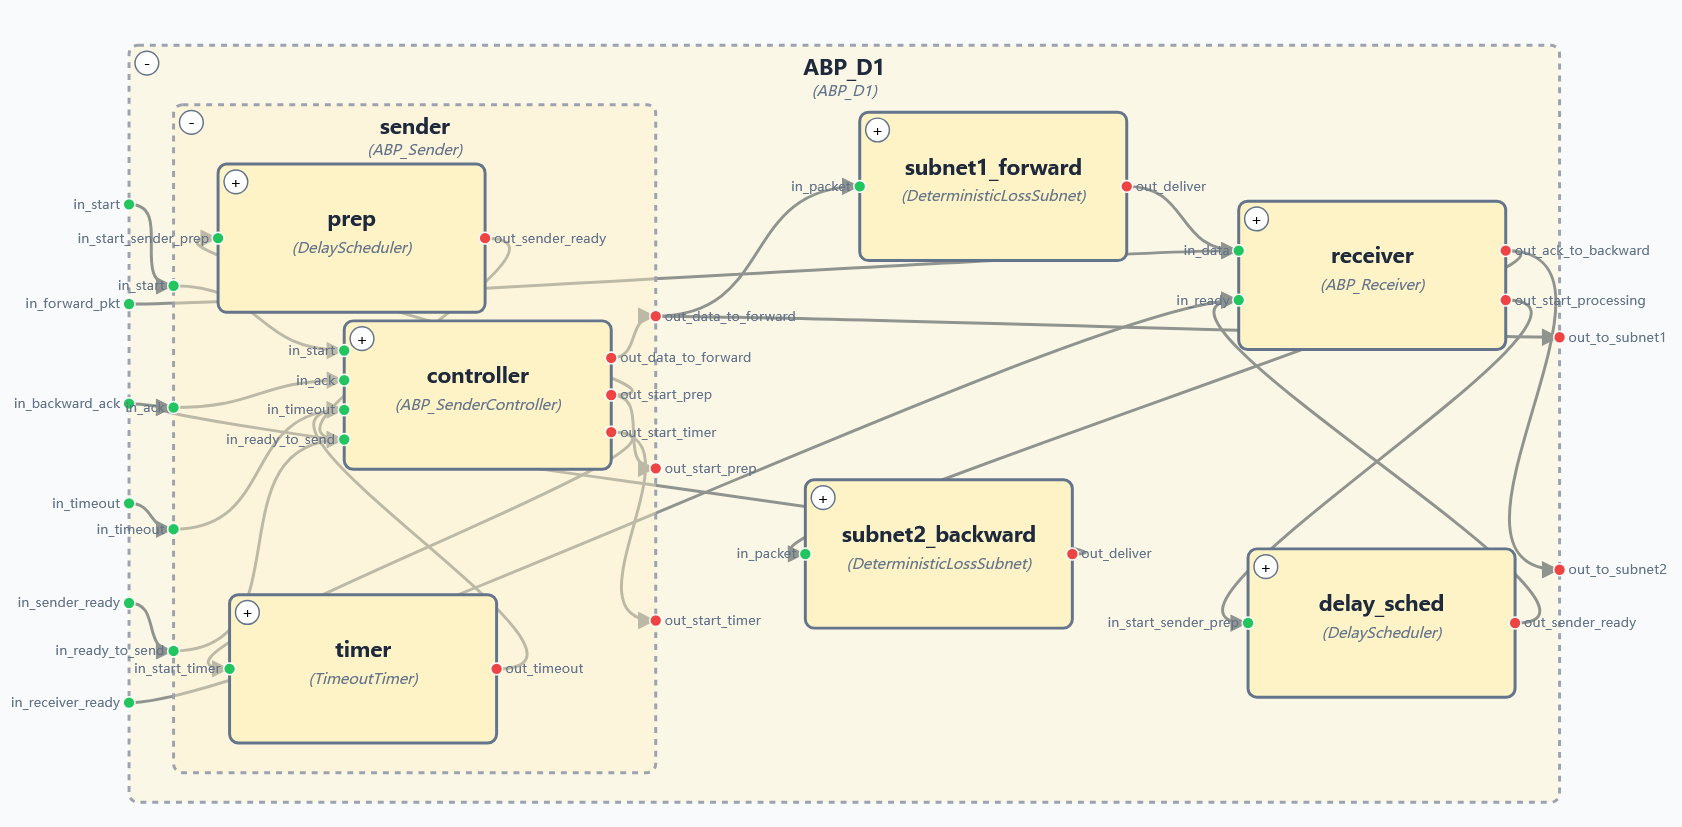
\includegraphics[width=0.99\textwidth]{imgs/ABP_model.png}
\caption{The final connection of the ABP DEVS model.}
\label{fig:code_graph}
\end{figure*}